\chapter{Results}
\label{chap:results}

In this section we will present our results. The results in the scientific part will be in relation to our research question and hypothesis. In the engineering part we will present how many of product goals we achieved at time of delivery. Different types of tests also go under this part. The final part is where we will show all our administrative results. This includes project planning, time sheets and documentation of our development process.

\section{Scientific Results}
The management API and deployment trigger may be protected from the internet in a self-hosted solution. By potentially operating on a physically separated network when this would be impractical or impossible in an external solution. The authors have also found that in an external solution it is necessary to trust the host with credentials giving them access to the environment APIs.


The count of each attack class in the hypothetical external solution and self-hosted solution. Where $n$ is the number of environments managed by the \acrshort{CD} solution.
\begin{table}[ht]
    \begin{tabularx}{\textwidth}{|X|c|c|}
        \hline
        \textbf{Attack class}                  & \textbf{External} & \textbf{Self-hosted}\\ \hline \hline
        open\_TCP/UDP-socket                   & 0 & 0        \\ \hline
        open\_TCP/UDP-socket                   & $1+n$ & $1+n$\\ \hline
        world-accessible\_TCP/UDP-socket       & $1+n$ & 0    \\ \hline
        open\_unsecured\_env-mgmt              & 0     & 0    \\ \hline
        open\_secured\_env-mgmt                & 0     & n    \\ \hline
        world\_accessible\_secured\_env-mgmt   & n     & 0    \\ \hline
        third-party\_credentials               & n     & 0    \\ \hline
        world-accessible\_deployment-trigger   & 1     & 0    \\ \hline
        locally-accessible\_deployment-trigger & 1     & 1    \\ \hline
    \end{tabularx}
    \caption{The number of times each attack class appears in the solutions}
    \label{tab:result1}
\end{table}

The the weighted sum, estimating the attack surface, of the hypothetical external solution and self-hosted solution.
\begin{table}[ht]
    \begin{tabularx}{\textwidth}{|X|c|c|}
        \hline
        \textbf{Solution}  & \textbf{Attack surface} & \textbf{Sum}\\ \hline \hline
        External           & $0.3\times(1+n) + 0.4\times(1+n) + 0.3\times n + n + 0.6 + 0.4$ & $2n + 1.7$\\ \hline
        Self-hosted        & $0.3\times(1+n) + 0.2\times(n) + 0.4$ & $(n + 1.4)/2$\\ \hline
    \end{tabularx}
    \caption{The attack surfaces of the solutions}
    \label{tab:result1}
\end{table}

\begin{center}
    \begin{figure}
        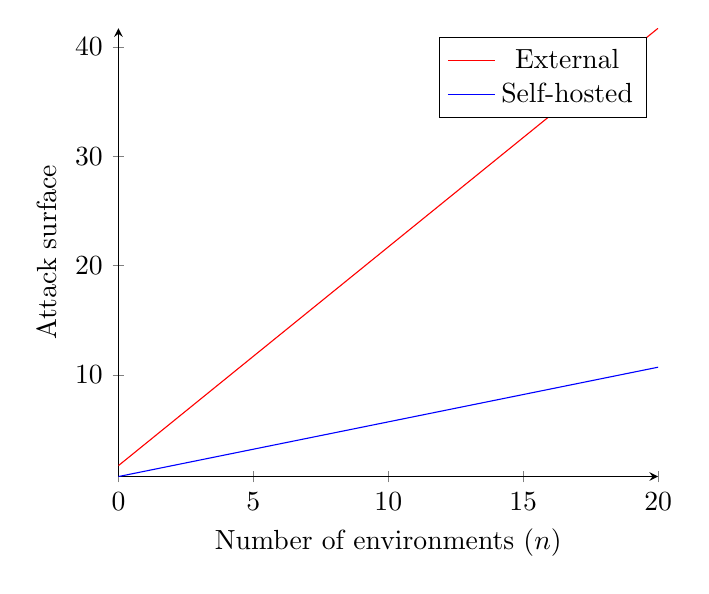
\begin{tikzpicture}
        \begin{axis}[
            axis lines = left,
            xlabel = {Number of environments ($n$)},
            ylabel = {Attack surface},
        ]
        %Below the red parabola is defined
        \addplot [
            domain=0:20, 
            samples=100, 
            color=red,
        ]
        {2*x + 1.7};
        \addlegendentry{External}
        %Here the blue parabloa is defined
        \addplot [
            domain=0:20, 
            samples=100, 
            color=blue,
            ]
            {0.5*x + 0.7};
        \addlegendentry{Self-hosted}
        \end{axis}
        \end{tikzpicture}
        \caption{Attack surface graph}
        \label{fig:my_label}
    \end{figure}
\end{center}

\section{Engineering Results}
% Planned features where implemented

% The feature implementation to add support for cion to deploy to Kubernetes turned out to be pretty simple compared to docker. This due to how Kubernetes requires
\subsection{Kubernetes support}
Kubernetes support was a highly regarded feature and was implemented as specified in the requirements document. Cion now has the ability to manage services in Kubernetes environments.


\subsection{Webhooks (Post-deploy behaviour)}
A new page that has been added to the web UI is the Webhooks page, it is used to configure the new webhook-feature. This feature allows the user to configure webhooks to trigger on specific events within the cion solution, for example when cion receives a new image or when a service is updated. 
Webhooks are highly configurable, thought this comes at the cost of them being complicated to configure, and does require a low-level understanding of the cion solution if the user wants to do something complicated. Though this is explained thoroughly in the end-user documentation. The complete list of configuration-options for webhooks is:

\begin{itemize}
    \item URL
    \item Headers
    \item Event
    \item Filters/triggers
    \item Body
\end{itemize}

The \textbf{URL} is the URL the webhook will send the \textit{POST}-request to.

The \textbf{headers} are what HTTP-headers to send to the URL.

The \textbf{event}-field is a select-box. The user has to select one, for example \textit{service-update}. 
When an event of the type selected occurs cion will run the events data through all the configured \textbf{filters}. The filters are regex-patterns that all have to match for the webhook to be fired. A filter is configured with a name and a value. The name is the name of the field in the event data, and the value is the regex-pattern that has to match that data for the filter to pass.

The \textbf{body} is the body of the HTTP-request to send to the configured URL. It supports the python format-function. So the user can insert fields from the event data into the body by using curly brackets around field-names in the text. For example:

\begin{verbatim}
    {{
        "service-name": "{service-name}"
    }}
\end{verbatim}

The above example generates a JSON-body containing exactly one key-value-pair, containing the service-name extracted from the event data. 
The user has to escape curly brackets, as shown above, due to how python's format-function tries to interpret them as variable-names.
The above body-string would result in the following when the field "service-name" in the event data is "cion\_api":

\begin{verbatim}
    {
        "service-name": "cion_api"
    }
\end{verbatim}

This example used JSON as the content type, but any string and formatting is supported. 

\subsection{Environments}
A new page was added where the user can configure and add environments for their cion instance to manage. It supports adding Kubernetes environments, and docker environments over TLS or the docker socket.


\subsection{Permissions}
A permissions system was implemented to allow administrators specify what features of cion a user should have access to. The admin can permit or deny access to service configuration on specific environments, environment configuration and cion-features like user-administration and log- and configuration-viewing.


\subsection{User settings/profile page}
The \textit{user settings}-, now named the \textit{profile}-page is implemented as specified in the requirements document. With fields to change the logged in user's password and gravatar-email. The user will only be able to change the password if they enter their old password. After changing their password they are logged out.

\subsection{Service update scheduling (Scheduled deployment)}
The individual service page has gotten an upgrade and a new feature was added, service update scheduling. It allows users to schedule the updating of a service to a specific time and date.


\section{Administrative Results}
%Skriv om måloppfyllelse i forhold til framdriftsplan: Planen, slik den var tidlig i prosjektet, og virkeligheten. (Eventuelle kommentarer og forklaringer på at ting ble som de ble, skal skrives i neste kapittel.)

%Timeregnskap, samlet fordelt på timeforbruk og aktiviteter. Referer til kalendertid dersom det er relevant.

%Studenter med systemutviklingsprosjekt må dokumentere at utviklingsprosessen de har valgt virkelig er brukt, ved å beskrive hva som har skjedd når og til hvilke tidspunkter. Detaljene legges i vedlegg. For tyngre prosesser skal de enkelte trinnene framgå av timelister og statusrapporter. For smidige utviklingsprosesser må dere bruke fantasien når det gjelder å dokumentere: User stories, sprints, filmer, bilder av tavler er aktuelle muligheter.

\subsection{Goal Achievement}
%WORK IN PROGRESS
There were several deviations from our original project plan. Partly because we over-estimated some parts, and under-estimated others. We also did not consider the mandatory work in February in our first project plan, which meant we had to push some features down the line. The biggest deviations were for Kubernetes support and scheduled deployment. We severely underestimated the hours needed to integrate Kubernetes support, but this was partly balanced out by overestimating the hours needed to implement scheduled deployment. Kubernetes support was planned for finalisation by the end March, but ended up being finished in late April. Meanwhile scheduled delivery was due the middle of April but was already done at the start of March. The important dates chapter in the project plan contain the original planned due dates.
%HUSK OG ENDRE TIMEANSLAG OG GANT DIAGRAM PLZZZZZZ
%Discuss how we did compared to our project plan

\subsection{Process}
%Discuss how we went about development
Our development process was a mixture of several different agile methods with tweaks and adjustments. We used parts of SCRUM. We skipped daily stand-up meetings, but we did have weekly meetings with the product owner.  We used a SCRUM-board on Atlassian's Jira to manage and track tasks. We decided as a team to have core hours between 10.00-15.00 from Monday through Friday. Sprints was also a part of SCRUM we dropped. Even though we did not use sprints, we did work in an iterative manner. Every meeting with the product owner gave us more feedback that either changed or created tasks on our SCRUM-board.


\subsection{Documentation}
%Discuss how we documented, where it can be read and why we did it like we did.
Most of the documentation for cion is written in markdown\cite{github-markdown} formatting. This allows it to be hosted on sites like github.com and readthedocs.io. Hosting on github makes the documentation accessible for the target users for cion, which are developers and system administrators. Github is a development platform to host and review code and manage projects\cite{github}, most developers already have a relationship to it.
